\documentclass[amsmath,amssymb,aps,nofootinbib,notitlepage,superscriptaddress]{revtex4-1}%
\usepackage{hyperref}
\usepackage{graphicx}
\usepackage[table]{xcolor}
\usepackage{latexsym}
\usepackage[normalem]{ulem}
\usepackage{bm}

%\documentclass[11pt]{amsart}
%\usepackage{geometry}                % See geometry.pdf to learn the layout options. There are lots.
%\geometry{letterpaper}                   % ... or a4paper or a5paper or ... 
%\usepackage{graphicx}
%\usepackage{amssymb}
%\usepackage{epstopdf}
%\DeclareGraphicsRule{.tif}{png}{.png}{`convert #1 `dirname #1`/`basename #1 .tif`.png}

\begin{document}


\title{Deriving Pearl's instrumental inequalities using the inflation DAG technique}
%\author{The Author}
\date{April 23, 2016}                                           % Activate to display a given date or no date
\maketitle


%\section{}
%\subsection{}

The instrumental inequality is a constraint for the DAG depicted in Fig. 8.1 of Pearl's book, reproduced here as Fig.~\ref{fig1}(a).  Consider the inflation DAG depicted in Fig.~\ref{fig1}(b).

\begin{figure}[h!]
\centering
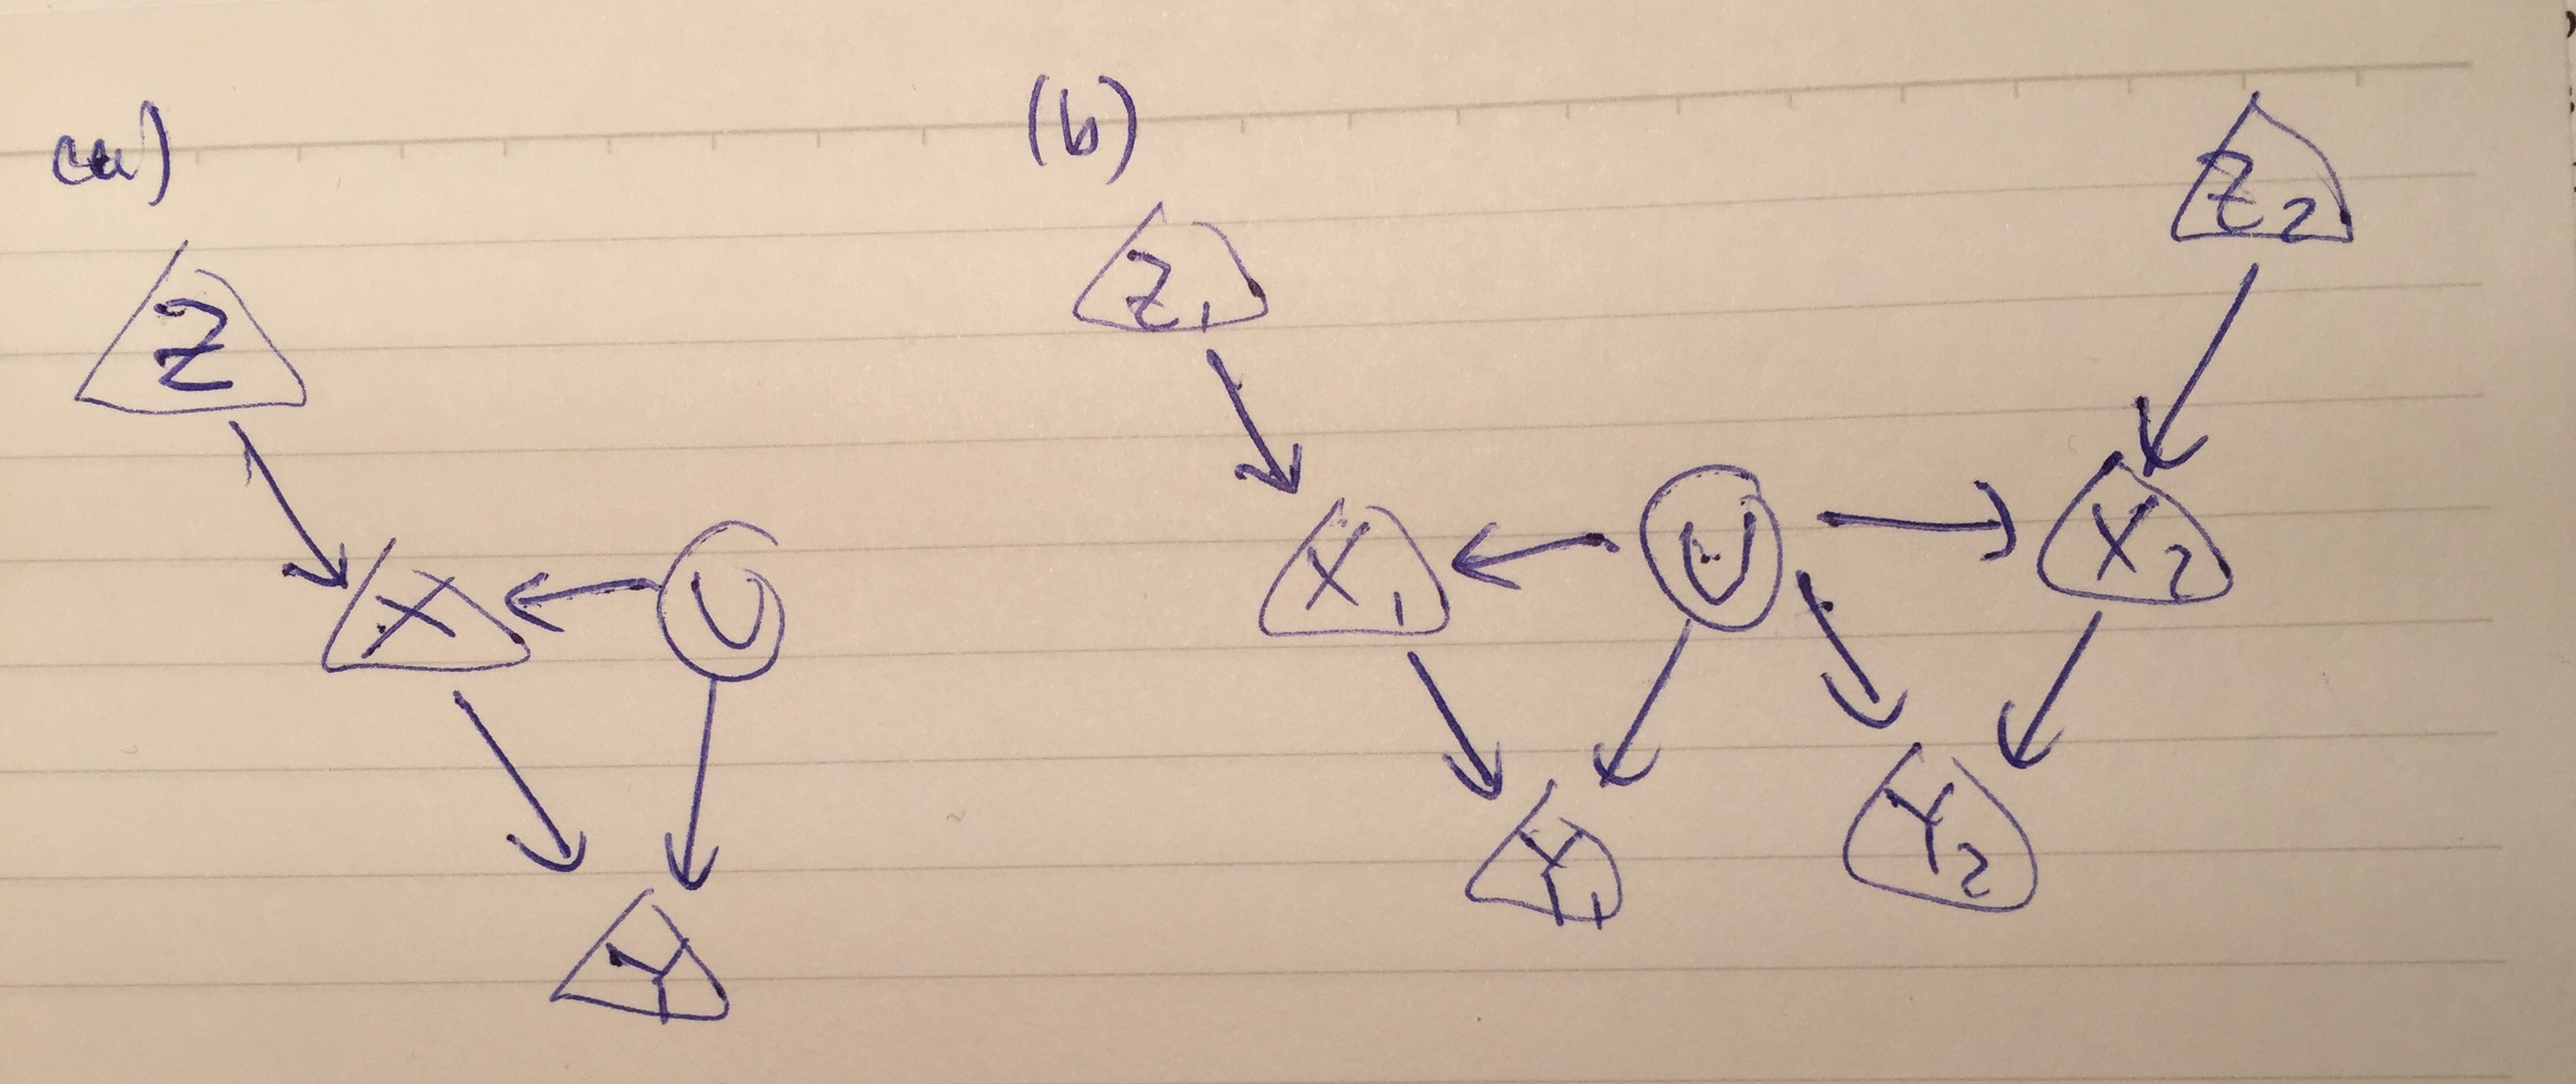
\includegraphics[scale=0.08]{InstrumentalDAG.jpg}
\label{fig1}
\end{figure}


Noting that the ancestral subgraph of $\{ Z_1 Z_2 X_1 Y_1\}$ is isomorphic to that of $\{ Z_1 Z_2 X_2 Y_2\}$, we can conclude that the associated distributions are equal,
\begin{align}\label{equiv}
P_{Z_1 Z_2 X_1 Y_1}= P_{Z_1 Z_2 X_2 Y_2}.
\end{align}

Now note that for any pair of values $a$, $b$,
\begin{align}
P_{Z_1 Z_2}(a,b) &= \sum_{c,d} P_{Z_1 Z_2 X_1 Y_1}(a,b,c,d),
\end{align}
which implies that for any value of $c$,
\begin{align}
 \sum_{d} P_{Z_1 Z_2 X_1 Y_1}(a,b,c,d) \le P_{Z_1 Z_2}(a,b).
\end{align}
As one concrete example, we can take $(a,b,c)= (0,1,0)$, in which case we obtain
\begin{align}
P_{Z_1 Z_2 X_1 Y_1}(0,1,0,0) + P_{Z_1 Z_2 X_1 Y_1}(0,1,0,1) \le P_{Z_1 Z_2}(0,1) .
\end{align}
Next comes the critical step.  We use Eq.~\eqref{equiv} to rewrite the second term on the LHS, thereby obtaining
\begin{align}
P_{Z_1 Z_2 X_1 Y_1}(0,1,0,0) + P_{Z_1 Z_2 X_2 Y_2}(0,1,0,1)\le P_{Z_1 Z_2}(0,1).
\end{align}
%as $P_{Z_1 Z_2 X_2 Y_2}(0,1,0,1)$.
Finally, we use the marginal independence relations implied by the inflation DAG to infer that
\begin{align}
&P_{Z_1 Z_2}(0,1)= P_{Z_1}(0)P_{Z_2}(1),\nonumber\\
&P_{Z_1 Z_2 X_1 Y_1}(0,1,0,0) = P_{Z_1 X_1 Y_1}(0,0,0) P_{Z_2}(1),\nonumber\\
&P_{Z_1 Z_2 X_2 Y_2}(0,1,0,1) = P_{Z_2 X_2 Y_2}(1,0,1)P_{Z_1 }(0).
\end{align}
This yields 
\begin{align}
P_{Z_1 X_1 Y_1}(0,0,0) P_{Z_2}(1) + P_{Z_2 X_2 Y_2}(1,0,1)P_{Z_1 }(0) &\le  P_{Z_1}(0) P_{Z_2}(1).
\end{align}
Finally, noting that the terms of this inequality refer only to injectable sets, we can infer that on the original DAG we have
\begin{align}
P_{Z X Y}(0,0,0) P_{Z}(1) + P_{Z X Y}(1,0,1)P_{Z }(0) &\le  P_{Z}(0) P_{Z}(1),
\end{align}
which is equivalent to 
\begin{align}
P_{X Y|Z}(0,0|0)  + P_{X Y|Z}(0,1|1) &\le  1,
\end{align}
which is an example of one of Pearl's instrumental inequalities (Eq.~8.21 in Pearl's book). 

\end{document}  